\let\negmedspace\undefined
\let\negthickspace\undefined
\documentclass[journal]{IEEEtran}
\usepackage[a5paper, margin=10mm, onecolumn]{geometry}
%\usepackage{lmodern} % Ensure lmodern is loaded for pdflatex
\usepackage{tfrupee} % Include tfrupee package

\setlength{\headheight}{1cm} % Set the height of the header box
\setlength{\headsep}{0mm}     % Set the distance between the header box and the top of the text

\usepackage{gvv-book}
\usepackage{gvv}
\usepackage{cite}
\usepackage{amsmath,amssymb,amsfonts,amsthm}
\usepackage{algorithmic}
\usepackage{graphicx}
\usepackage{textcomp}
\usepackage{xcolor}
\usepackage{txfonts}
\usepackage{listings}
\usepackage{enumitem}
\usepackage{mathtools}
\usepackage{gensymb}
\usepackage{comment}
\usepackage[breaklinks=true]{hyperref}
\usepackage{tkz-euclide} 
\usepackage{listings}
% \usepackage{gvv}                                        
\def\inputGnumericTable{}                                 
\usepackage[latin1]{inputenc}                                
\usepackage{color}                                            
\usepackage{array}                                            
\usepackage{longtable}                                       
\usepackage{calc}                                             
\usepackage{multirow}                                         
\usepackage{hhline}                                           
\usepackage{ifthen}                                           
\usepackage{lscape}
\begin{document}

\bibliographystyle{IEEEtran}
\vspace{3cm}

\title{1.1.7.2}
\author{EE24BTECH11039 - Mandala Ranjith
}
% \maketitle
% \newpage
% \bigskip
{\let\newpage\relax\maketitle}

\renewcommand{\thefigure}{\theenumi}
\renewcommand{\thetable}{\theenumi}
\setlength{\intextsep}{10pt} % Space between text and floats


\numberwithin{equation}{enumi}
\numberwithin{figure}{enumi}
\renewcommand{\thetable}{\theenumi}


\textbf{Question}:x\\
The points $\brak{1,2}$ , $\brak{0,0}$ and $\brak{a,6}$ are collinear
\\ \textbf{Solution: }\\
    \begin{table}[h!]    
      \centering
      \input{tables/tab1.tex}
      \caption{}
    \end{table}\\
\begin{align}
\textbf Performing row operation on \text{M} \\
\textbf{M'}=  \myvec{1&a\\0&6-2a} \\
\textbf for $\text{A},\text{B},\textbf{C}$ to be collinear \\ rank\brak{\text{M}}=1\\
 $6-2a=0$ \\
 $a=3$ \\
\end{align}

    \begin{figure}[h]
        \centering
       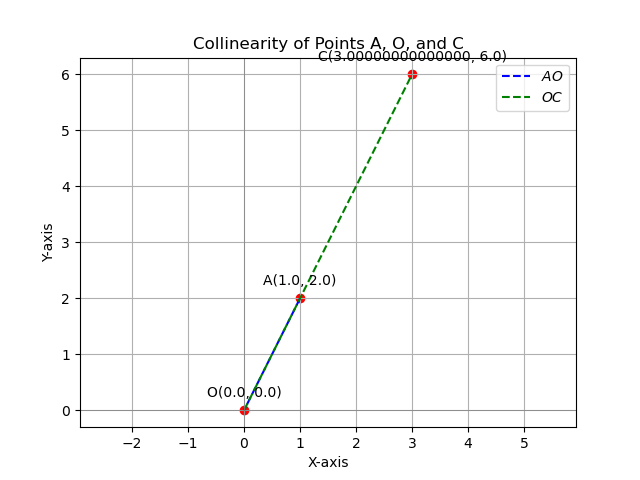
\includegraphics[width=0.7\linewidth]{figs/fig1.png}
       \caption{}
       \label{graph}
    \end{figure}



\end{document}
